\chapter{Oide effect}
This part of the document addresses the radiation phenomena called Oide effect\cite{Oide}, which sets a limit on the beam size demagnification, specially important in linear collider because of the strong focusing required in the Final Doublet before the Interation Point (IP).\par
First, a brief introduction to the beam size limit (Oide limit) is given, where adittional calculations have been derived to include this radiation phenomenon in the lattice design and optimization. The Oide effect is evaluated for the CLIC 3 TeV and CLIC 500 GeV parameters, leading to change the length of the first quadrupole before the IP, called QD0. It ends with a proposal to mitigate the impact of the strong focusing by adding correctors before and after the QD0, recovering part of the luminosity.\par
\section{Beam size limit}\label{Oideeffect}
The Oide effect is caused by the interaction of charged particles with the magnetic field from quadrupoles. Radiation in a focusing magnet, schematically represented as QD0 in Fig. (\ref{f:Oideeffect}), changes the energy of the particle and limits the focusing effect upstream the Interaction Point (IP). This imposes a limit on the minimum beam size specially relevant in the vertical plane.\par%For the horizontal direction, is mainly affected by radiation caused by the interaction of charged particles with the magnetic field from dipoles. %This report will be limited to sector dipoles or ``sbends''.\par
\begin{figure}[!hbt]
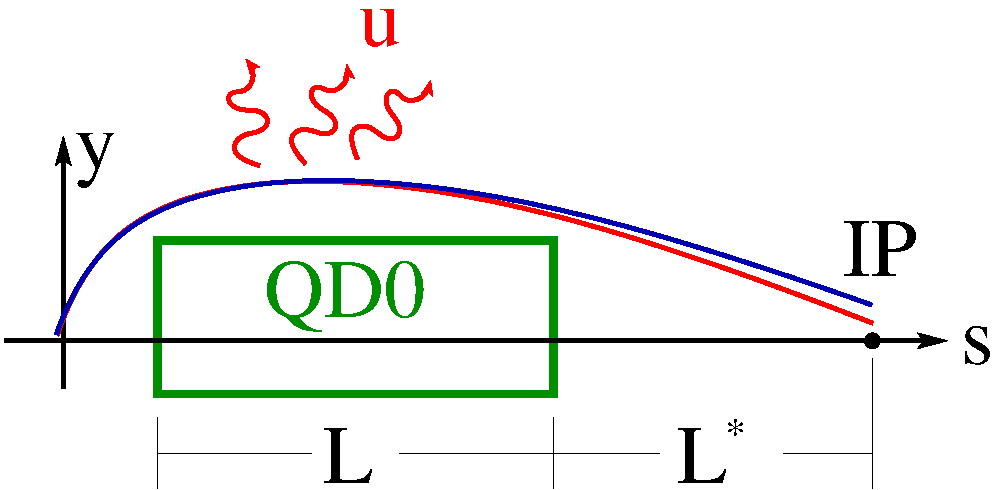
\includegraphics[scale=0.5]{Oide.pdf}
\centering
\caption{Designed particle trajectory in blue and the trajectory of a particle due to radiation in the quadrupole in red.}\label{f:Oideeffect}
\end{figure}
 The beam size growth due to radiation is added quadratically to the linear beam size $\sigma_0^2=\epsilon\beta$ where $\beta$ is optical beta function and $\epsilon$ is the emittance. Therefore, $ \sigma^2 = \sigma_0^2 + \sigma_{oide}^2$, and the beam size contribution is,
 \begin{equation}
  \sigma^2_{oide} = \frac{110}{3\sqrt{6\pi}}r_e\frac{\lambda_e}{2\pi}\gamma^5 F(\sqrt{k}L,\sqrt{k}L^*)\left(\frac{\epsilon}{\beta^*}\right)^{5/2}
  \label{Oideequ}
 \end{equation}
 where
 \begin{equation}
  F(\sqrt{k}L, \sqrt{k}L^*) = \int_0^{\sqrt{k}L}|\sin\phi+\sqrt{k}L^*\cos\phi|^3\left[\int_0^\phi(\sin\phi'+\sqrt{k}L^*\cos\phi')^2 d\phi'\right]^2d\phi
  \label{OideF}
 \end{equation}
  and $\lambda_e$ is the Compton wavelength of the electron, $r_e$ is the classical electron radius, $\gamma$ is the relativistic factor, $\epsilon$ is the geometrical beam emittance, $\beta^*$ is the Twiss parameter at the observation point (in this case, the IP), and $k$, $L$ and $L^*$ are the quadrupole gradient, the quadrupole length and the distance to the observation point measured from the closest magnet face.\par
   Although the total contribution to beam size depends on lattice and beam parameters, the minimum achievable beam size is given by
%the function $F$ is calculated only from quadrupole parameters. For this reason, $F$ will be used as figure of merit for a quadrupole.
\begin{equation}
 \sigma_{y \text{ min}} = \left(\frac{7}{5}\right)^\frac{1}{2}\left[\frac{275}{3\sqrt{6\pi}}r_e\frac{\lambda_e}{2\pi}F(\sqrt{K}L,\sqrt{K}L^*)\right]^\frac{1}{7}(\epsilon_{Ny})^\frac{5}{7}
\end{equation}
where $\epsilon_N=\gamma\epsilon$ is the normalized emittance, showing the independence from beam energy.\par
 
\subsection{Double integral solution}
 The double integral used to calculate $F$ has been solved with the goal to increase the computational calculation speed. The inner integral over $\phi'$ can be solved because it has a known primitive.
\begin{equation}
 \int_0^\phi (\sin \phi'+ \sqrt{k}l^*\cos\phi')^2d\phi'=\frac{\phi}{2}[(\sqrt{k}l^*)^2 +1 ] + \frac{\sin(2\phi)}{4}[(\sqrt{k}l^*)^2 -1]+\sqrt{k}l^*\sin^2\phi
\end{equation}
The Eq. (\ref{OideF}) can now be expressed as one integral.
{\scriptsize
\begin{align}
F(\sqrt{k}L&,\sqrt{k}l^*) =\\
&\int_0^{ \sqrt{k}L} |\sin\phi+\sqrt{k}l^*\cos\phi|^3 \left( \frac{\phi}{2}[(\sqrt{k}l^*)^2 +1 ] + \frac{\sin(2\phi)}{4}[(\sqrt{k}l^*)^2 -1]+\sqrt{k}l^*\sin^2\phi\right)^2 d\phi\notag
\end{align}
}
The squared factor in brackets is always positive because all inner terms are real. The term inside the absolute value is also always positive, therefore, the integrand is always positive. Now, considering the function:
  \begin{equation}
  |\sin \phi + \sqrt{k}l^*\cos\phi|=\left\{
  \begin{array}{c l l}
&  \sin\phi+\sqrt{k}l^*\cos	\phi,\quad\qquad&\text{if}, \sin\phi+	\sqrt{k}l^*\cos	\phi\geq0\\
&  -(\sin\phi+\sqrt{k}l^*\cos\phi),\quad&\text{if}, \sin\phi+	\sqrt{k}l^*\cos	\phi<0
  \end{array}\right.\label{eq-absval}
 \end{equation}
sign changes at every point $\quad\phi_n = \arctan(-\sqrt{ k}l^*)\pm n\pi,\quad n\geq1$.\par
It is possible to split the integration interval $i$ times, being $i$ the number of $\phi_n$ solutions where $0<\phi_n<\sqrt{k}L$. On each of those intervals, the absolute value definition can be removed and replaced by the corresponding expression in Eq. (\ref{eq-absval}), having only a difference in sign. By defining the primitive $\mathscr{F}$ in an interval where the factor inside the absolute value is positive it is possible to evaluate $F$ as it is shown in Eq. (\ref{eq-primeval}).
\begin{equation}
 F(\sqrt{k}L,\sqrt{k}l^*)= \mathscr{F}|_0^{\phi_1} - \mathscr{F}|_{\phi_1}^{\phi_2} +  \mathscr{F}|_{\phi_2}^{\phi_3} - \mathscr{F}|_{\phi_3}^{\phi_4}+ \cdots \pm  \mathscr{F}|_{\phi_i}^{\sqrt{k}L}\label{eq-primeval}
\end{equation}
The change of signs in each interval is only  given by the absolute value definition, then, it is simpler to add the absolute value of each contribution.
\begin{equation}
 F(\sqrt{k}L,\sqrt{k}l^*)= \bigr\vert\mathscr{F}|_0^{\phi_1}\bigr\vert + \bigr\vert\mathscr{F}|_{\phi_1}^{\phi_2}\bigr\vert +  \bigr\vert\mathscr{F}|_{\phi_2}^{\phi_3}\bigr\vert + \bigr\vert\mathscr{F}|_{\phi_3}^{\phi_4}\bigr\vert + \cdots +\bigr\vert\mathscr{F}|_{\phi_i}^{\sqrt{k}L}\bigr\vert
\end{equation}
If we know the primitive $\mathscr{F}$ and we are able to calculate the $\phi_n$s in the integration interval, then, it is possible to calculate the factor $F$ without using an approximate integrator. The double integration has been simplified to a primitive evaluation.
\clearpage

\subsection{The primitive \texorpdfstring{$\mathscr{F}$}{F}}
The primitive $\mathscr{F}$ exists and it has been calculated using Maxima \cite{Maxima} and Wolfram Alpha Mathematica\cite{Wolfram} software.
 \begin{align*}
  \mathscr{F}&=\frac{1}{1209600.0} \{1323 \cos(5\sqrt{k}L)-675 \cos(7\sqrt{k}L)\\
        &\hspace{1cm}+\sqrt{k}L (378000 \sin(\sqrt{k}L)+21000 \sin(3\sqrt{k}L)-7560 \sin(5\sqrt{k}L))\\
        &\hspace{0.5cm}+\sqrt{k}l^* [23625 \sin(\sqrt{k}L)+4725 \sin(3\sqrt{k}L)-14175 \sin(5\sqrt{k}L)+4725 \sin(7\sqrt{k}L)\\
        &\hspace{1cm}+\sqrt{k}L  (-37800 \cos(5\sqrt{k}L))\\
        &\hspace{1cm}+(\sqrt{k}L)^2 (-75600 \sin(3\sqrt{k}L)+226800 \sin(\sqrt{k}L))]\\
        &\hspace{0.5cm}+(\sqrt{k}l^*)^2 [-49707 \cos(5\sqrt{k}L)+14175 \cos(7\sqrt{k}L)\\
        &\hspace{1cm}+\sqrt{k}L  (1587600 \sin(\sqrt{k}L)-172200 \sin(3\sqrt{k}L)+68040 \sin(5\sqrt{k}L))]\\
        &\hspace{0.5cm}+(\sqrt{k}l^*)^3 [-80325 \sin(\sqrt{k}L)-144725 \sin(3\sqrt{k}L)+82215 \sin(5\sqrt{k}L)-23625 \sin(7\sqrt{k}L)\\
        &\hspace{1cm}+\sqrt{k}L  (37800 \cos(5\sqrt{k}L))\\
        &\hspace{1cm}+(\sqrt{k}L)^2 (680400 \sin(\sqrt{k}L)-126000 \sin(3\sqrt{k}L))]\\
        &\hspace{0.5cm}+(\sqrt{k}l^*)^4 [68985 \cos(5\sqrt{k}L)-23625 \cos(\sqrt{k}L)\\
        &\hspace{1cm}+\sqrt{k}L  (2041200 \sin(\sqrt{k}L)-205800 \sin(3\sqrt{k}L)+37800 \sin(5\sqrt{k}L))]\\
        &\hspace{0.5cm}+(\sqrt{k}l^*)^5 [-458325 \sin(\sqrt{k}L)-43225 \sin(3\sqrt{k}L)-25893 \sin(5\sqrt{k}L)+14175 \sin(7\sqrt{k}L)\\
        &\hspace{1cm}     +\sqrt{k}L  (68040 \cos(5\sqrt{k}L))\\
        &\hspace{1cm}     +(\sqrt{k}L)^2 (680400 \sin(\sqrt{k}L)-25200 \sin(3\sqrt{k}L))]\\
        &\hspace{0.5cm}+(\sqrt{k}l^*)^6 [-945 \cos(5\sqrt{k}L)+4725 \cos(7\sqrt{k}L)\\
        &\hspace{1cm}     +\sqrt{k}L  (831600 \sin(\sqrt{k}L)-12600 \sin(3\sqrt{k}L)-37800 \sin(5\sqrt{k}L))]\\
        &\hspace{0.5cm}+(\sqrt{k}l^*)^7 [(-354375) \sin(\sqrt{k}L) + 5425 \sin(3\sqrt{k}L)-1323 \sin(5\sqrt{k}L)-675 \sin(7\sqrt{k}L)\\
        &\hspace{1cm}+\sqrt{k}L  (-7560 \cos(5\sqrt{k}L))\\
        &\hspace{1cm}+(\sqrt{k}L)^2 (226800 \sin(\sqrt{k}L) + 25200 \sin(3\sqrt{k}L))]\\
        &\hspace{0.5cm}+\cos(\sqrt{k}L) ((\sqrt{k}l^*)^2+1)(4725)[(\sqrt{k}l^*)^5(\sqrt{k}L)(80)\\
        &\hspace{1cm}     +(\sqrt{k}l^*)^4 (155-48(\sqrt{k}L)^2)\\
        &\hspace{1cm}     +(\sqrt{k}l^*)^3 (\sqrt{k}L)(64)\\
        &\hspace{1cm}     +(\sqrt{k}l^*)^2 (182-96 (\sqrt{k}L)^2)\\
        &\hspace{1cm}     +\sqrt{k}l^*  (-16 \sqrt{k}L)\\
        &\hspace{1cm}     +(\sqrt{k}L)^2 (-48)+75]\\
        &\hspace{0.5cm}+\cos(3\sqrt{k}L) (-175) [(\sqrt{k}l^*)^7 (\sqrt{k}L) (120)\\
        &\hspace{1cm}    +(\sqrt{k}l^*)^6(3)(144(\sqrt{k}L)^2+71)\\
        &\hspace{1cm}    +(\sqrt{k}l^*)^5 (\sqrt{k}L) (744)\\
        &\hspace{1cm}    +(\sqrt{k}l^*)^4 (720(\sqrt{k}L)^2+347)\\
        &\hspace{1cm}    +(\sqrt{k}l^*)^3 (\sqrt{k}L)(-24)\\
        &\hspace{1cm}    +(\sqrt{k}l^*)^2 (144 (\sqrt{k}L)^2-473)\\
        &\hspace{1cm}    +\sqrt{k}l^* (-648) \sqrt{k}L\\
        &\hspace{1cm}    +(\sqrt{k}L)^2 (-144)-31]\}
 \end{align*}

This equation was included in MapClass2\cite{Mapclassorig,Mapclass,Mapclass2,githubMapClass2}.\par In order to confirm that the code implementation gave the same result than the original double integral, random values were assigned to $\sqrt{k}l^*$ and $\sqrt{k}L$ and both expressions, the solved and the double integral, were numerically evaluated with difference lower than $10^{-3}$ relative.\par

\section{Oide Beam size contribution}
\begin{table}[!hbt]
\centering
\begin{tabular}{l||c|c|c||c|c|c|c|c||c|c}\hline\hline
Lattice &$\epsilon_N$& $\gamma$& $\sigma_0$&$k$&$L$&$L^*$& $F$ & $\sigma_{oide}$&$\sigma$&$\sigma_{min}$\\
 &(nm)&($10^3$)&(nm)&(m$^{-2}$)&(m)&(m)&&(nm) &(nm)&(nm)\\\hline
CLIC 3 TeV & 20 & 2935.0 & 0.70 & 0.116 & 2.73 &3.5&  4.086  & 0.85 & 1.10& 1.00 \\
CLIC 500 GeV & 25 & $\;\;$489.2 & 2.3 & 0.077 & 3.35 &4.3& 4.115 & 0.08 & 2.3 & 1.17\\
ILC  500 GeV & 40 & $\;\;$489.2 & 5.7 & 0.170 & 2.20 &4.3& 9.567 & 0.04 & 5.7 & 1.85\\\hline
\end{tabular}\caption{Vertical beam size and radiation beam size contribution for three lattices. $\epsilon_N$ is the normalized emittance, $\epsilon_N=\gamma\epsilon$.}\label{t:Sigmas}
\end{table}
% \begin{table}[hbt]
% \centering
% \begin{tabular}{l||c|c|c||c|c|c|c||c}\hline\hline
% Lattice &$\epsilon_N$& $\gamma$& $\sigma_0$&$k$&$L$&$l^*$& $F$ & $\sigma_{oide}$\\
%  &(nm)&($10^3$)&(nm)&(m$^{-2}$)&(m)&(m)&&(nm)\\\hline
% CLIC 3 TeV & 20 & 2935.0 & 0.7 & 0.116 & 2.73 &3.5&  4.086  & 0.85\\
% CLIC 500 GeV & 25 & $\;\;$489.2 & 2.3 & 0.077 & 3.35 &4.3& 4.115 & 0.08\\
% ILC  500 GeV & 40 & $\;\;$489.2 & 5.7 & 0.170 & 2.20 &4.3& 9.567 & 0.04\\\hline
% \end{tabular}\caption{Beam size and radiation beam size contribution for three lattices. $\epsilon_N$ is the normalized emittance.}\label{tabSigmas}
% \end{table}\par
The Oide beam size contribution depends on combination of beam and optics parameters. %Table \ref{tabSigmas} gives the results.
If none of the beam parameters is to be changed then $F$ can be used as a figure of merit of the optics as it is calculated only from $k$, $L$ and $l^*$. The target is to reduce it as much as possible and two energy cases are analyzed: 3 TeV ($l^*=3.5$ m) and 500 GeV ($l^*=4.3$ m).\par
Columns $\sigma_0$, $\sigma_{oide}$ and $F$ in Table \ref{t:Sigmas} show that CLIC 3 TeV and 500 GeV \cite{CLICdes,TomasCLIC} have larger contributions to beam size even having a lower $F$ value than ILC 500 GeV \cite{ILCdes}.\par
In order to evaluate the minimum possible $F$ for $L$ and $l^*$ given, the minimum $k$ required to get the particles focused is when the Twiss function $\alpha$ is zero just at the quadrupole opposite face to the IP.\par
Fig. \ref{fig-3TeV:a}  shows the ratio squared between the beam size contribution due to Oide effect and the linear beam size for three cases: when $k$ is the minimum required to get particles focused (to get $\alpha_y=0$ at QD0 opposite side to the IP), when $k$ is calculated as thin lens ($k=\frac{1}{Ll^*}$), and the current QD0 status. Fig. \ref{fig-3TeV:b} shows the $k$ values for the previous mentioned cases.\par
The Oide contribution to beam size is of the same order of the linear beam size. It might be possible to reduce it by doubling the current quad length. Quad lengths larger than 10 m do not lead to further improvements with the current parameters.\par

\begin{figure}[tbh]
\centering
\begin{subfigure}{1.0\textwidth}
\centering
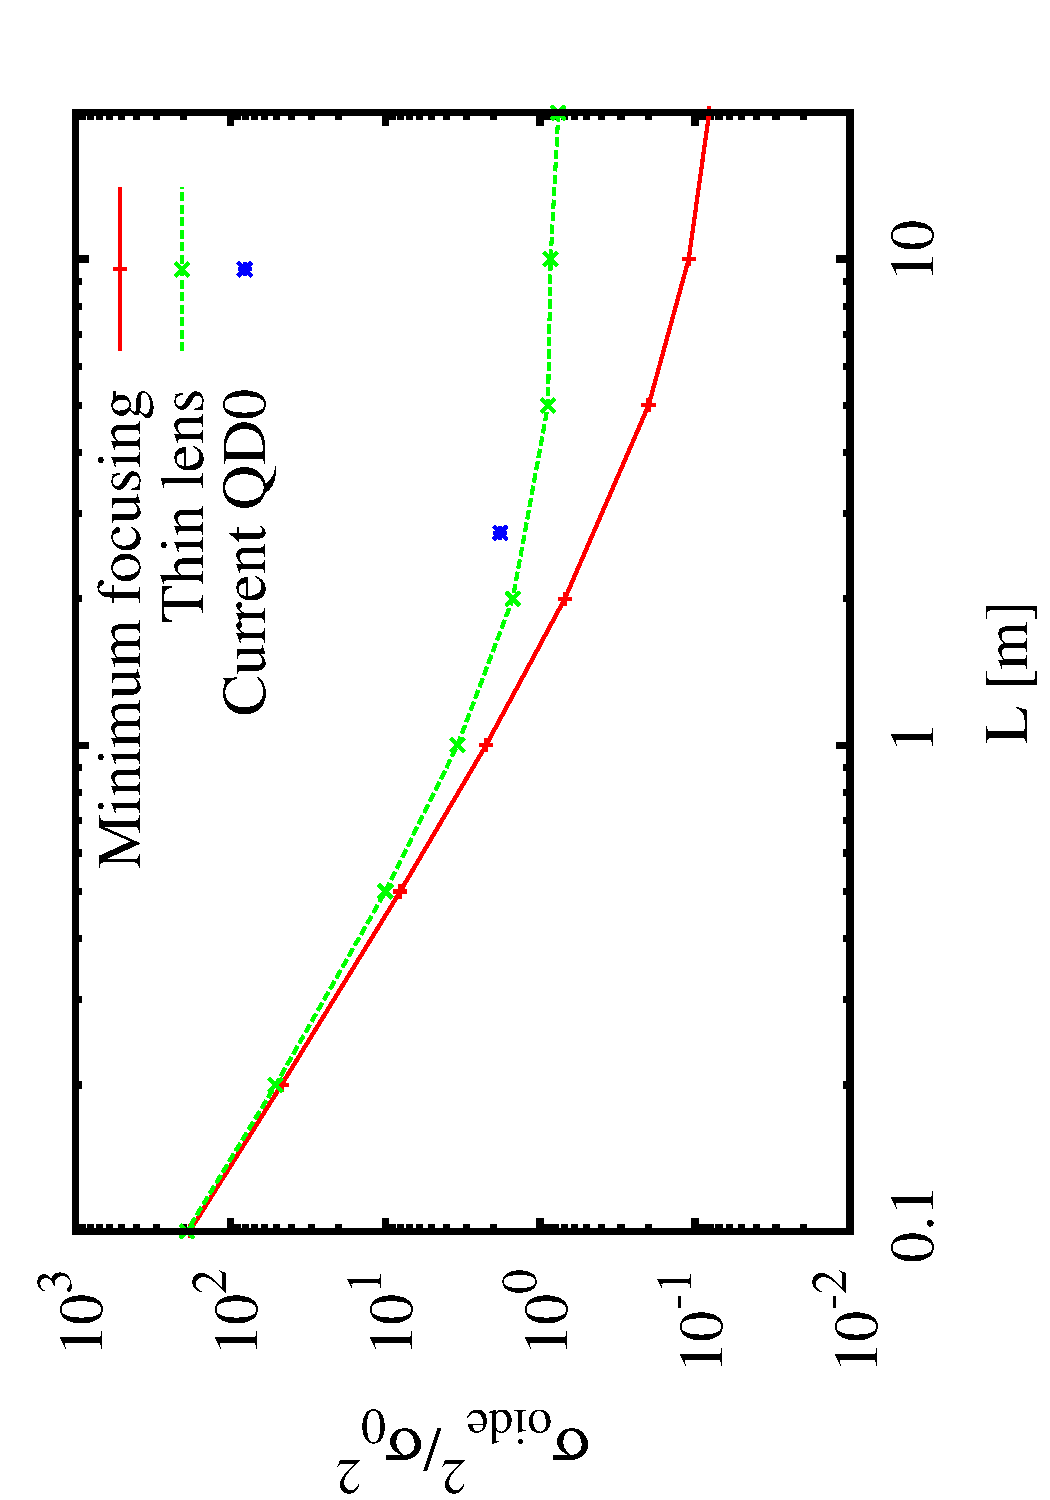
\includegraphics[scale=0.55,angle=-90]{image07a.pdf}\caption{}\label{fig-3TeV:a}
\end{subfigure}\par
\begin{subfigure}{1.0\textwidth}
\centering
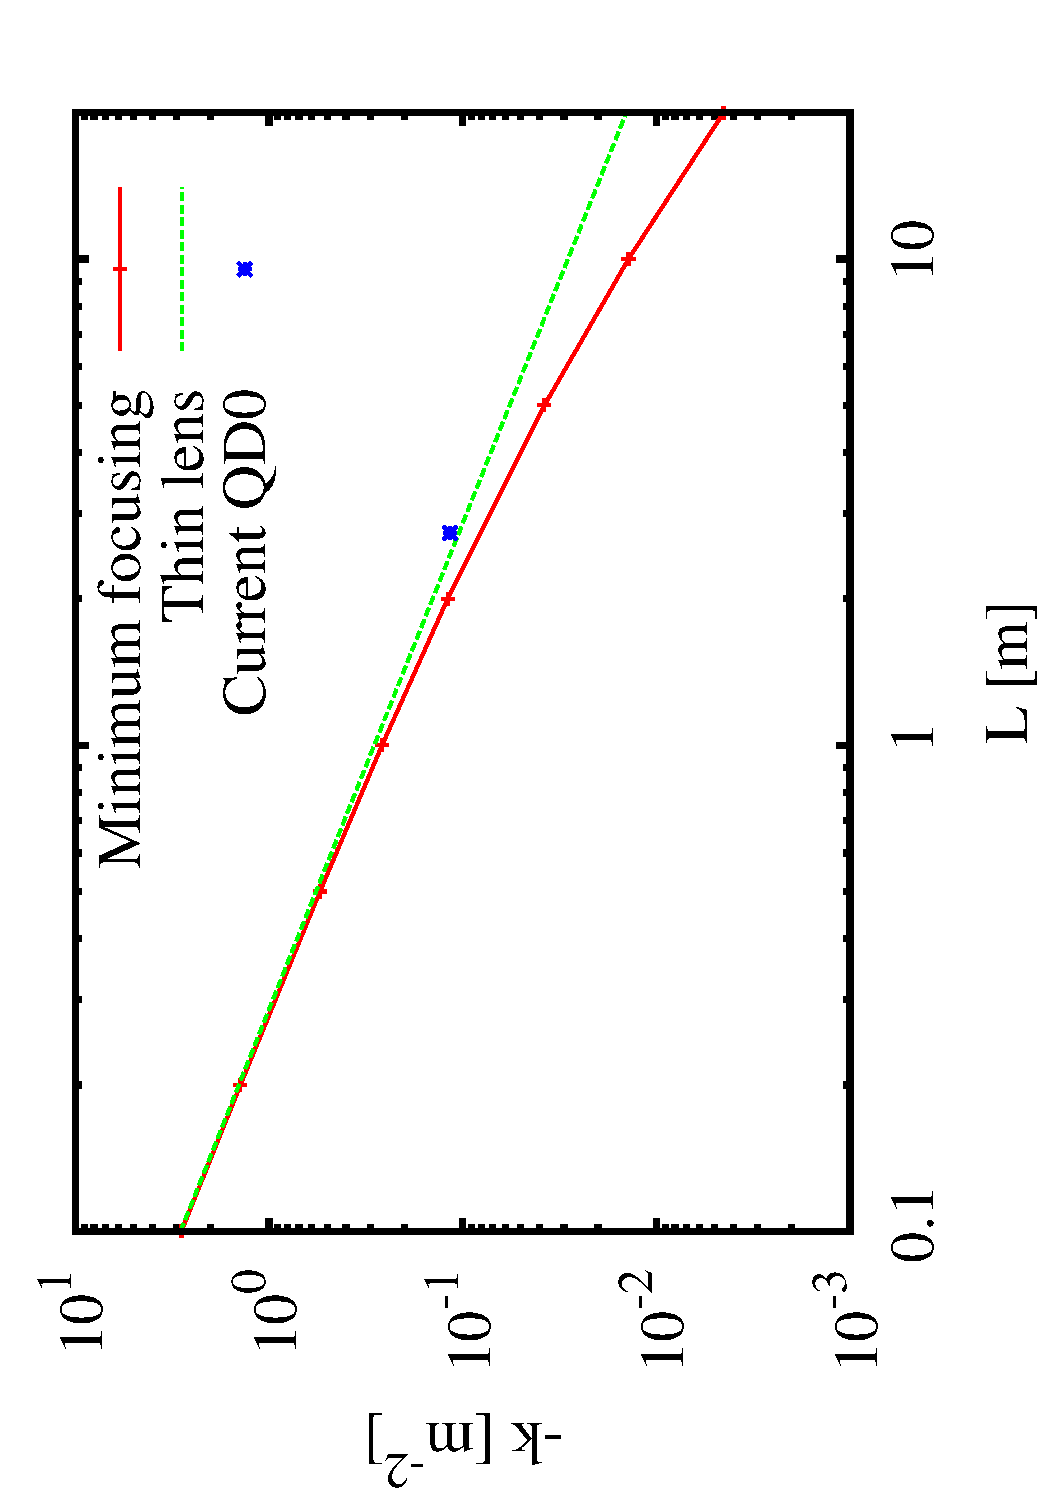
\includegraphics[scale=0.55,angle=-90]{image07b.pdf}\caption{}\label{fig-3TeV:b}
\end{subfigure}
\caption{Oide effect beam size contribution for CLIC 3 TeV design parameters. (a) $\sigma^2_{oide}$ normalized to designed linear beam size as a function of quad length for the minimum focusing $k$ (when $\alpha_y=0$ at the quadrupole opposite side to the IP), for $k$ calculated as thin lens ($k=\frac{1}{Ll^*}$) and the current QD0. (b) $k$ in the three previous cases for comparison.}\label{fig-3TeV}
 \end{figure}\par
Fig. \ref{fig-500GeV} is the corresponding to Fig. \ref{fig-3TeV} for the 500 GeV case. The current design contributes less than 4\% of the total beam size, concluding that the current QD0 length with the CLIC 500 GeV parameters does not need adjustment.\par
\begin{figure}[htb]
\centering
\begin{subfigure}{1.0\textwidth}
\centering
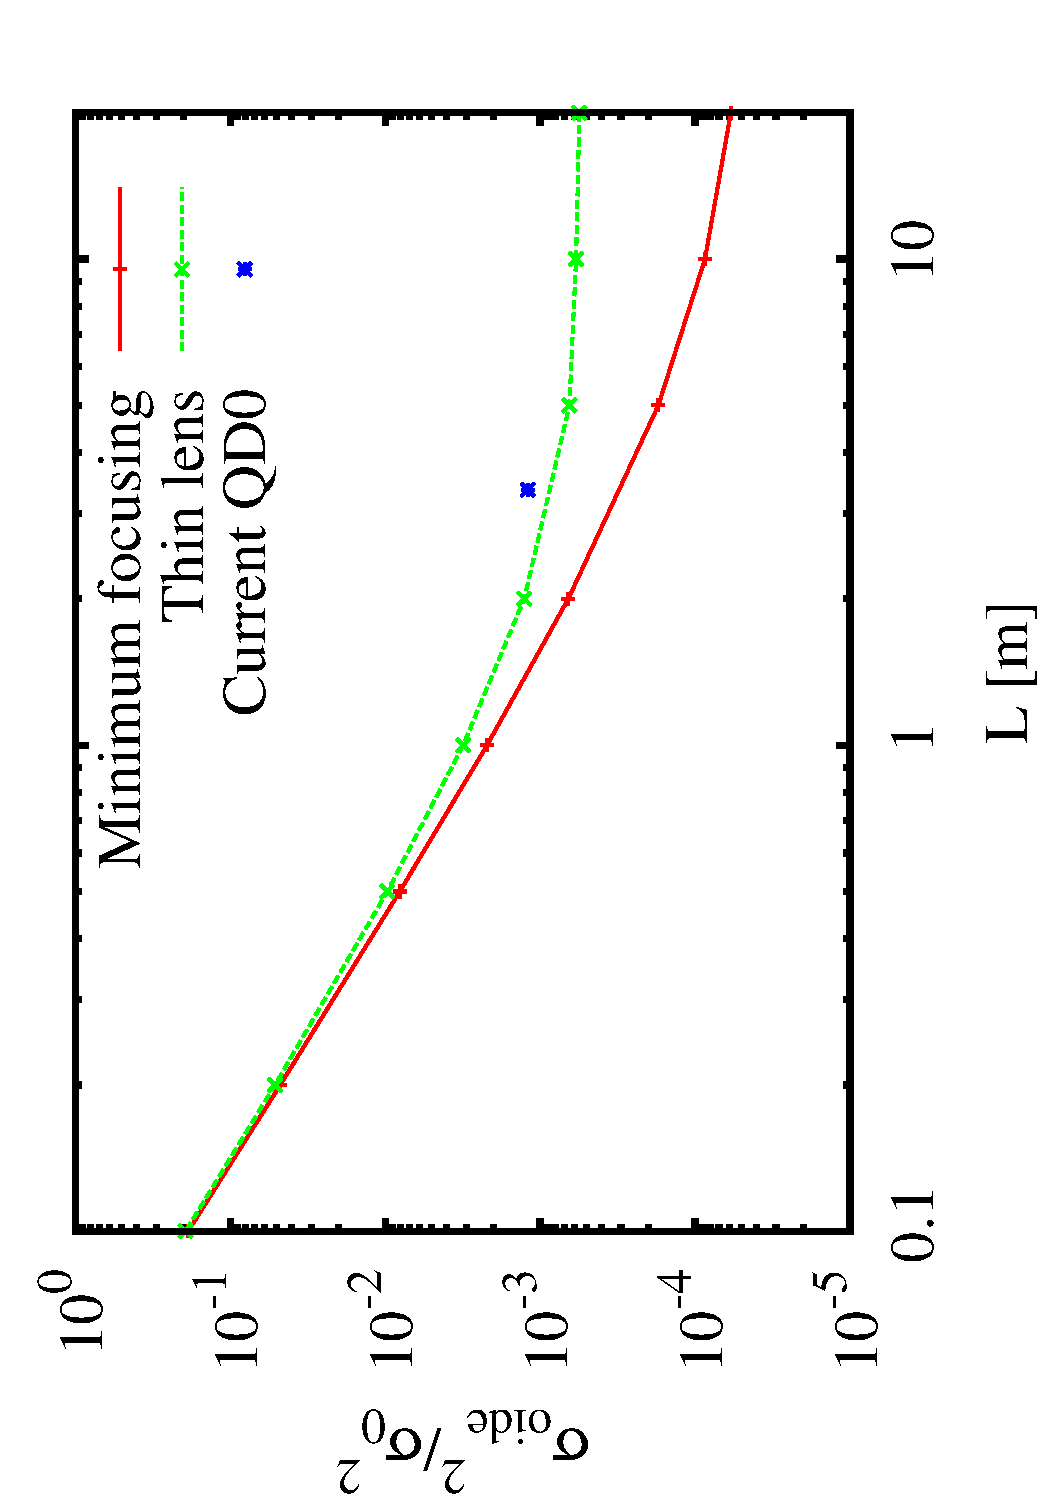
\includegraphics[scale=0.55,angle=-90]{image06b.pdf}\caption{}
\end{subfigure}
\begin{subfigure}{1.0\textwidth}
\centering
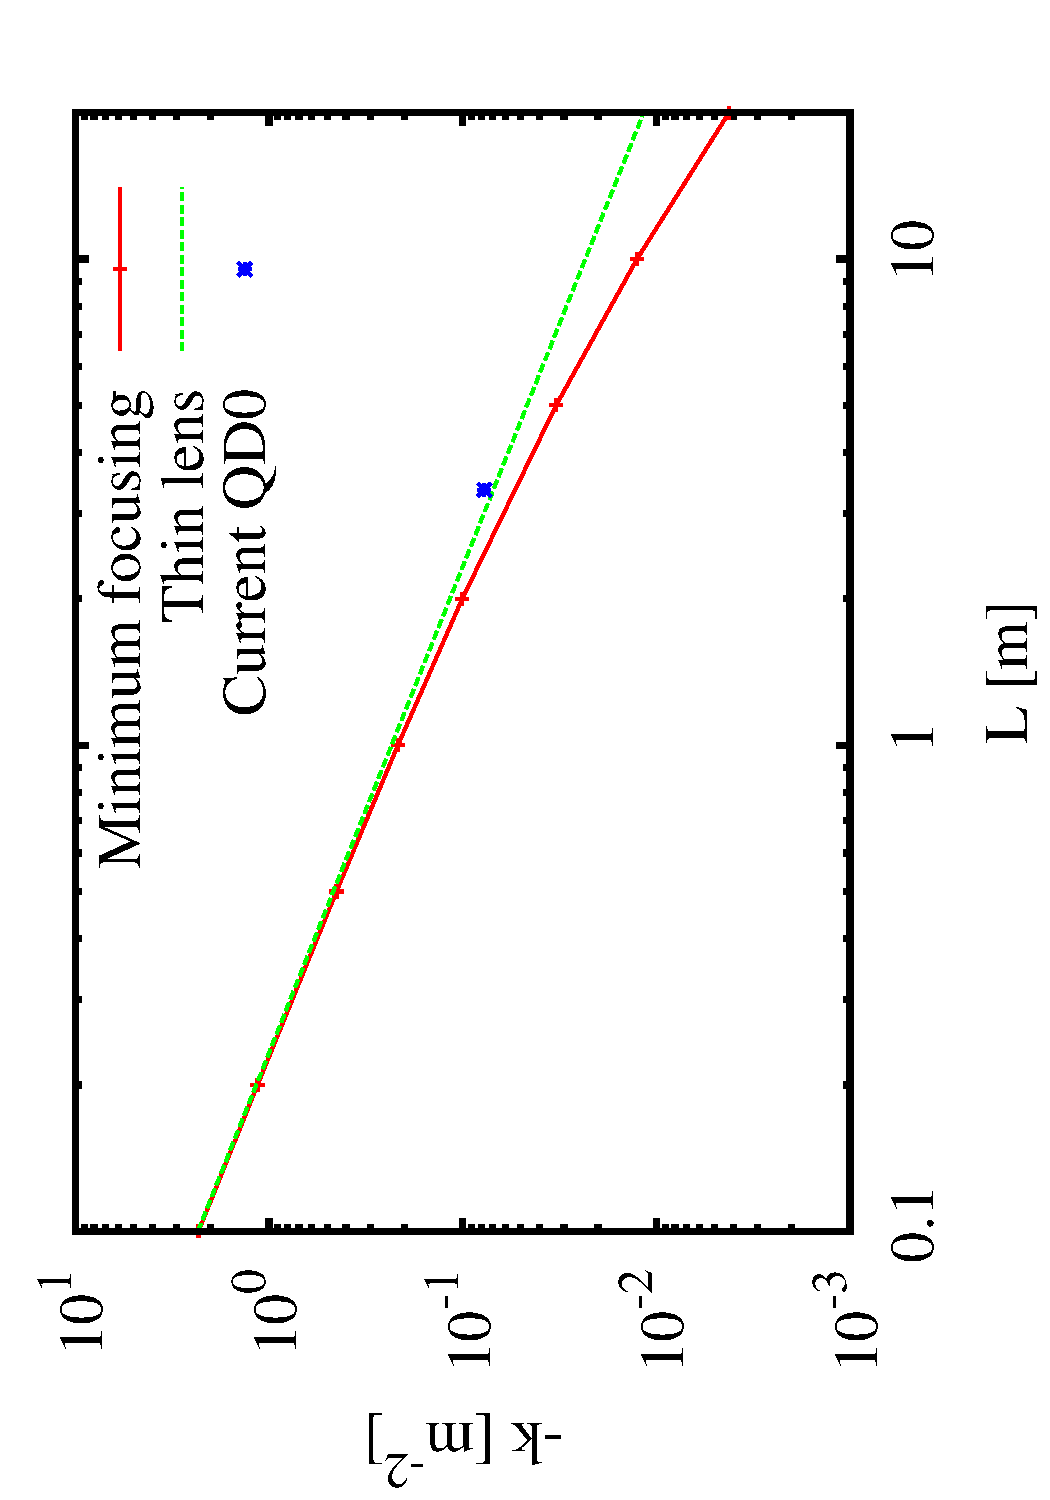
\includegraphics[scale=0.55,angle=-90]{image06c.pdf}\caption{}
\end{subfigure}
\caption{Oide effect beam size contribution for CLIC 500 GeV design parameters. (a) $\sigma^2_{oide}$ normalized to designed linear beam size as a function of quad length for the minimum focusing $k$ (when $\alpha_y=0$ at the quadrupole opposite side to the IP), for $k$ calculated as thin lens ($k=\frac{1}{Ll^*}$) and the current QD0. (b) $k$ in the three previous cases for comparison.}\label{fig-500GeV}
 \end{figure}\par
 
\section{Mitigation on the beam size impact}
\subsection{$\Delta y$ due to radiation}
Particle tracking from QD0 input to the IP for CLIC 3 TeV with and without radiation using PLACET \cite{Placet} gives the six dimentional phase space effect of radiation. Fig. (\ref{f:CLIC3TeVbeamsizeIP}) shows the current transversal distribution of particles. The ideal would be to remove $\Delta y = y_\text{rad} -y_0$.\par
\begin{figure}[!htb]
\centering
 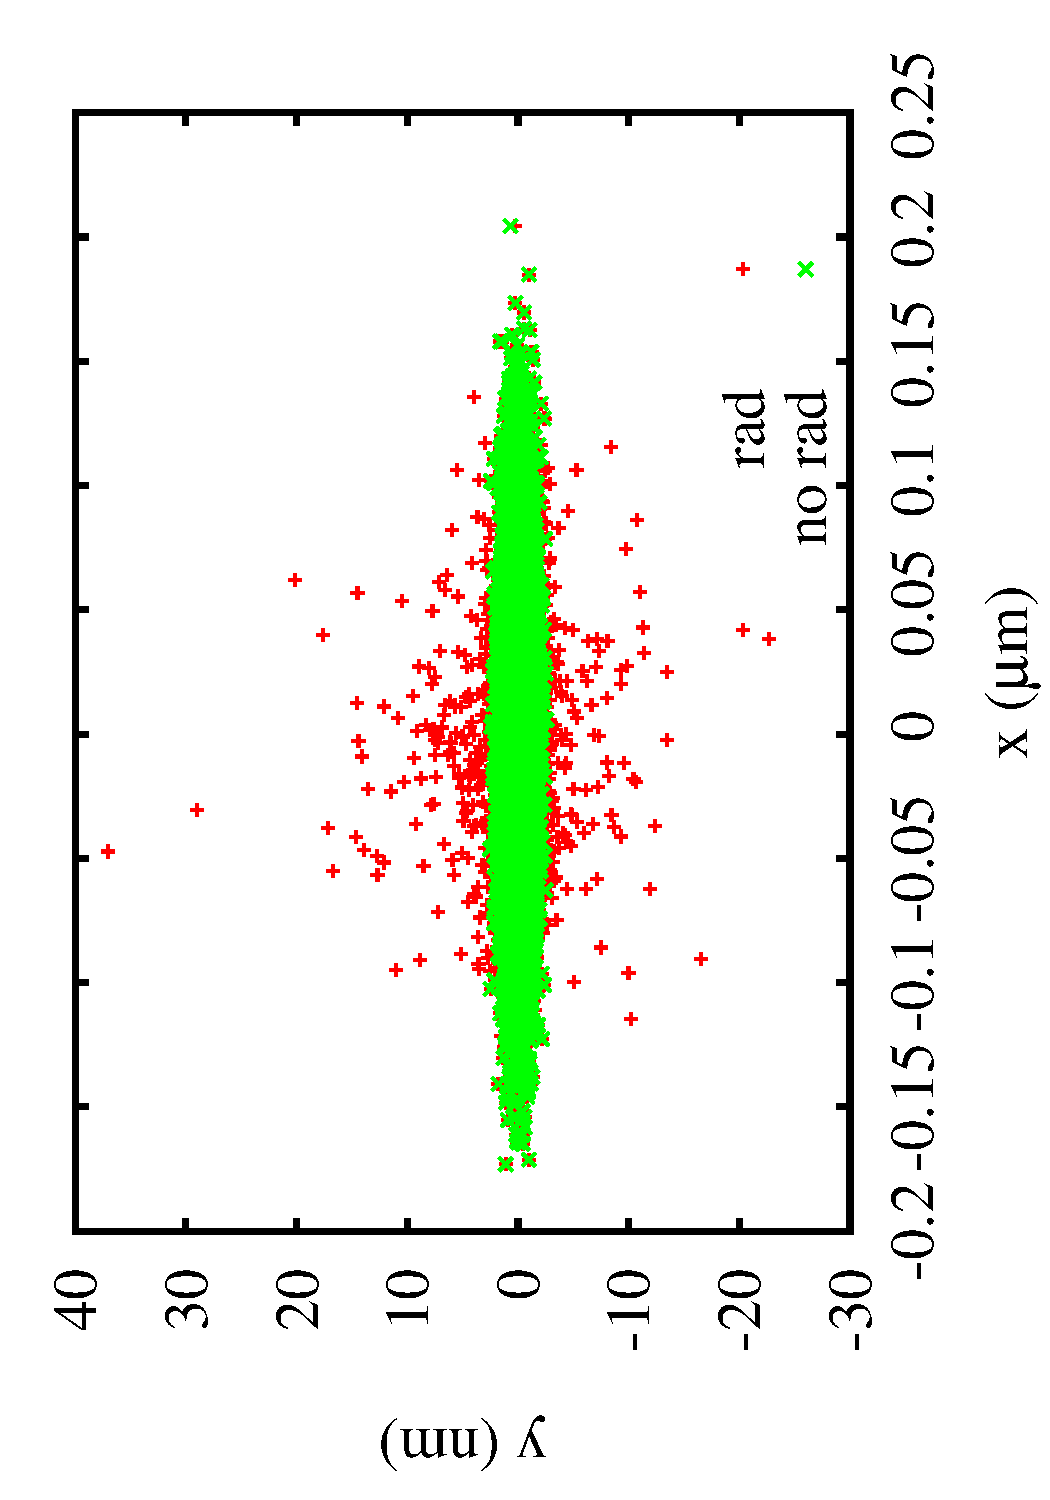
\includegraphics[scale=0.3,angle=-90]{plotxyrad.pdf}\caption{CLIC 3 TeV beam at the IP after tracking QD0 with and without radiation.}\label{f:CLIC3TeVbeamsizeIP}
\end{figure}
Oide averages over the phase space $u,s,y,y'$, being $u$ the energy of the photons radiated, $s$ the longitudinal coordinate, and $y,y'$ the vertical component and its derivative with respect to $s$, obtaining $\langle \Delta y \rangle = 0$. But this result hides a correlation between $\Delta y, y'$, %
\begin{equation}
 \langle\Delta y (y'_0)\rangle = \frac{2}{3}r_e\gamma^3G(\sqrt{K}L,\sqrt{K}L^*)(y'_0)^3
\end{equation}
%$r_e$ is the clasical electron radius and 
where $G(\sqrt{K}L,\sqrt{K}L^*)$ is
{\scriptsize
\begin{equation}
\int_0^{\sqrt{K}L}(\sin\phi+\sqrt{K}L^*\cos\phi)^2\int_0^\phi (\sin\phi'+\sqrt{K}L^*\cos\phi')^2 d\phi'd\phi
\end{equation}
}
Fig. (\ref{f:correlation}) shows the comparison between the correlation obtained from tracking and the theoretical evaluation of the previous expression.
\begin{figure}[!htb]
\centering
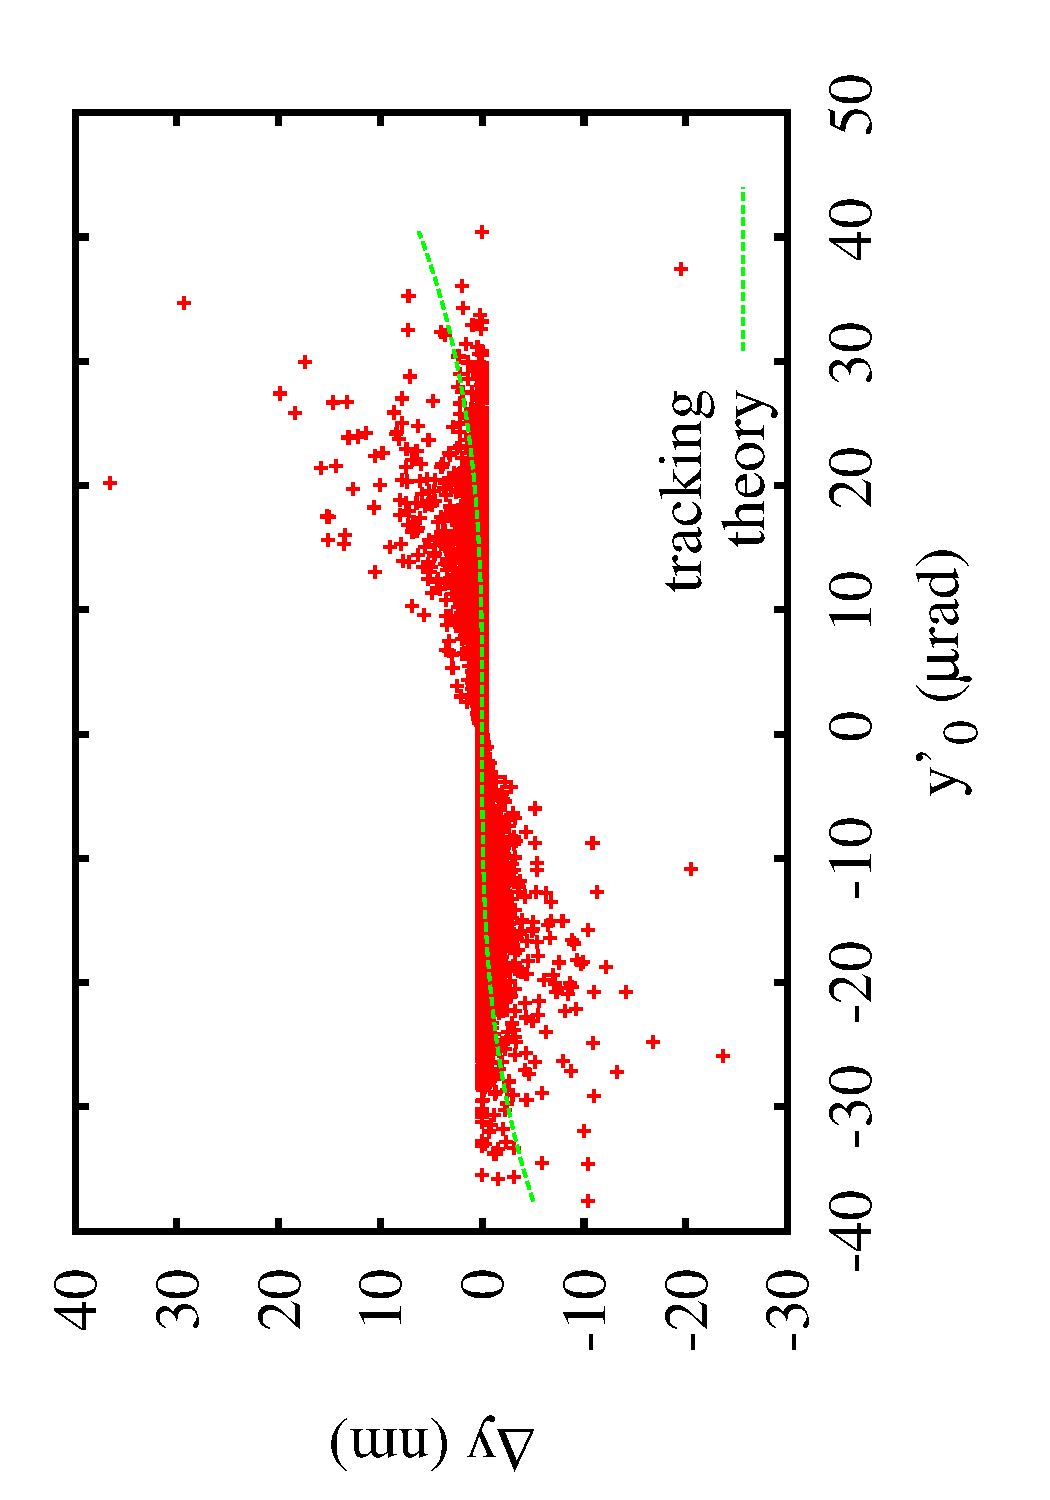
\includegraphics[scale=0.3,angle=-90]{plotdyrad.pdf}\caption{Correlation between the phase space coordinates $y,y'$ for CLIC 3 TeV from particle tracking and theoretical expression.}\label{f:correlation}
\end{figure}

\subsection{Corrector}
A pair of correctors, as in Fig. (\ref{f:corrector}), is added to the strong focusing in order to mitigate the radiation effect. Procedure consist in : first, scan the best position and multipole gradient ($s,k_i$) for C0, and then set C1 at QD0 input to cancel the effect of C0.\par
\begin{figure}[!htb]
\centering
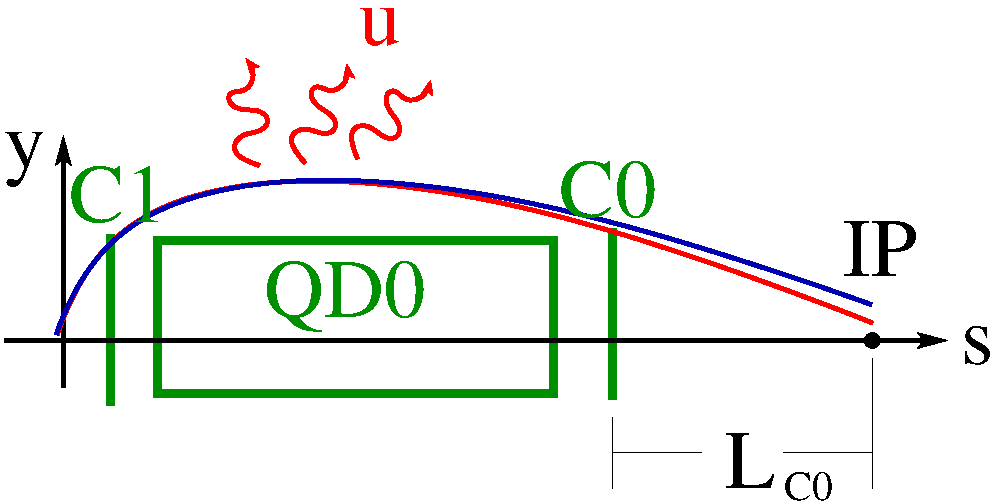
\includegraphics[scale=0.3,angle=0]{Oide2.pdf}\caption{Nominal trajectory in blue: the kick in C1 must cancel the kick in C0. All particles that radiate in red: the difference in kicks should cancel $\Delta y$.}\label{f:corrector}
\end{figure}
Two sets of correctors (C0,C1) where tried. Quadrupoles (QD00,QD01) to substract the equivalent of a linear fit, and Octupoles (OD0,OD1) for a cubic fit.
\begin{table}[!hbt]
\centering
\begin{tabular}{l||c|c|c}\hline\hline
Corrector & i & $L$ & $k_{i}$\\
& & (m)& (m$^{-(i+1)}$)\\\hline
QD00 & 1 & 0.01 &\\
QD01 & 1 & 0.01 &\\\hline
OD0 & 3 & 0.01 & 36\\
OD1 & 3 & 0.01 & 0\\\hline
\end{tabular}\caption{Correctors}\label{t:correctors}
\end{table}

\subsection{Limitations}
It was not possible to reduce the correlation more because even that C0 adds very little to radiation. But at some point the radiation in C1 starts to be important. It might be possible to scan  C1 ($s,k$) to find a place where it radiates less. Even with perfect C1 to C0 correction there will be a limit when radiation will affect the Horizontal plane. Here the target was set to less than 1\% of horizontal beam size increase. Mean correlation could be reduced to a minimum as there is not correlation per each particle... (other target?)

\subsection{Conclusions}
Radiation in the final quad sets a limit on the vertical beamsize, this is called Oide effect. Even if the mean value of the trajectory change is zero, there is a correlation between the change in trajectory and the angle at the IP due to the energy change. This correlation is reduced by correctors before and after QD0. The best result yet has been with octupoles giving a vertical beam size reduction of $(4.3\pm??)$\%
